\chapter{Helium}
\label{chap:he}
\section{Recent Developments}
    Calculation of very precise physical properties of helium is of interest in the field of metrology to develop accurate calibration and pressure standards, to accurately compute the Boltzmann constant, and to improve acoustic gas thermometry  \cite{Garberoglio2009,Fellmuth2006,Schmidt2007,Pitre2006,Moldover2010,Aziz1995}. Semi-classical virial coefficients up to fifth order have been computed for helium-4 by Shaul et al. \cite{Shaul2012SC}, and showed that first-principles properties could be evaluated with precision and accuracy that exceeds experiment. Garberoglio and Harvey \cite{Garberoglio2009,Garberoglio2011,Garberoglio2011b} reported fully quantum second and third virial coefficients for helium-3 and helium-4 including exchange effects where needed, for temperatures as low as 2.6K. Shaul et al. \cite{Shaul2012} reported fully quantum virial coefficients of helium-4 (but without exchange) up to fourth order for temperatures of T = 2.6~K -- 1000~K.
\section{Computational Details}
    In Sec. \ref{chap:methods:subsec:PI SCB} we noted that using different propagators brought about changes only in the effective potential used. While a given propagator will correspond to some effective potential, the converse might not necessarily be true -- selection of an \emph{ad hoc} effective potential might not map back to an appropriate propagator. Still, it may be interesting to examine other choices of semi-classical potential for use in a PIMC framework, without deriving it from a propagator. Once the accuracy of such an \emph{ad hoc} potential is established empirically, we can then compare its efficiency against the TI propagator. We have in mind in particular the QFH effective potential \cite{Feynman, Schenter2002},
    modified slightly for this purpose. We denote this as QFH* and it is given as:
    \begin{equation}\label{eq:QFHCh3}
        \begin{aligned}
            U_2^{\rm QFH^*} (\bm{r}_{1,i}, \bm{r}_{2,i}) &= U_2 (\bm{r}_{1,i}, \bm{r}_{2,i}) + \displaystyle\frac{\hbar^2 \beta}{24 m P^2} \Big[ \frac{\partial^2 U_2 (\bm{r}_{1,i}, \bm{r}_{2,i})}{\partial r_{12,i}^2} + \frac{2}{r_{12,i}}~\frac{\partial U_2 (\bm{r}_{1,i}, \bm{r}_{2,i})}{\partial r_{12,i}}  \Big],\\
            |r_{12,i}|^2 &= |\bm{r}_{1,i} - \bm{r}_{2,i}|^2
        \end{aligned}
    \end{equation}
    where $m$ is the mass of the atom. We use the $1/P^2$ prefactor for the second term as it closely resembles the TI propagator and also gives the best results of those we examined. The standard QFH semi-classical potential is obtained for $P = 1$.

    The \abinitio{} helium pair potential that we used is due to Przybytek et al. \cite{Przybytek2010} (denoted as $u$) and a simplified, approximate version of the same (denoted as $u^{\rm simple}$) was obtained from supplementary material of Shaul et al. \cite{Shaul2012}. We investigated a total of 8 temperatures ranging from $T$ = 2.5 K to 500 K. Mayer Sampling Monte Carlo (MSMC) \cite{Singh2004,Schultz2009}, which uses importance sampling to compute virial coefficients efficiently for any given interaction potential, was employed in our calculations.

    Since this work is aimed at extending the work of Shaul et al.~\cite{Shaul2012}, we shall be comparing the performance of the TI propagator and the QFH* effective potential against their results. In order to make a fair and consistent comparison, we employ the same decomposition algorithms as Shaul et al. \cite{Shaul2012}. These schemes were developed to improve the efficiency of the virial coefficient calculation, doing so by computing the full quantum virial coefficients through a series of stages of increasing accuracy in the quantum treatment and adherence to the target PES. We have the same three choices for the preliminary approximation: (1) semi-classical, $[\Gamma^{\rm SCL}(u)]$, (2) the $u^{\rm simple}$ approximation to the semi-classical treatment, $[\Gamma^{\rm SCL}(u^{\rm simple})]$ and (3) the $u^{\rm simple}$ approximation to $u$ for a finite $P$, $[\Gamma (P,u^{\rm simple})]$. Here $\Gamma$ represents the configurational integral of the associated potential, the square brackets indicate an independent simulation, and the superscript SCL denotes a QFH semi-classical approximation (Eq. \eqref{eq:QFH}) to $u$ or $u^{\rm simple}$. Since we are interested only in $B_2$, the Percus-Yevick compressibility route approximation\cite{Percus1958,Hansen,Shaul2011} to the semi-classical approximation is ignored.

    Any computational details regarding the inter-molecular potentials, decomposition strategies and MSMC parameters that are not included here may be found in Sec. B of Shaul et al. \cite{Shaul2012} and the supplementary material therein.
\section{Results and Discussion}
    For ease of reference and use, we note and define the following:
    \begin{itemize}
        \item All the simulations involved the same set of inter-molecular potentials, $u$ or $u^{\rm simple}$ or their semi-classical approximations.
        \item We denote quantum virial coefficient results from Shaul et al. \cite{Shaul2012} as $B_2^{\rm cl}$, those using the QFH* effective potential as $B_2^{\rm sc,QFH^*}$, and those using the TI propagator as $B_2^{\rm sc,TI}$; the first part of the superscript denotes which type of beads (classical (cl) or semi-classical (sc)) were used in the PIMC calculations. Note this is not to be confused with the preliminary approximations $[\Gamma^{\rm SCL} (u)]$ or $[\Gamma^{\rm SCL} (u^{\rm simple})]$ which denote the semi-classical calculations using the QFH approximations to $u$ and $u^{\rm simple}$ respectively.
        \item In the same spirit, we refer to the algorithm for computing $B_2^{\rm cl}$ as the Classical Beads approach denoted as CB; $B_2^{\rm sc,QFH^*}$ as the Semi-Classical Beads QFH* approach denoted as SCB-QFH*; $B_2^{\rm sc,TI}$ as the Semi-Classical Beads TI approach denoted as SCB-TI.
        \item It is possible to use a semi-classical TI approximation ($P = 1$ in Eq. \eqref{eq:TIworking}) instead of the QFH (Eq. \eqref{eq:QFH}) approximation while using the TI propagator. However, after performing several calculations, we observed that using semi-classical TI approximations as preliminary approximations always led to inefficient decompositions, which resulted in larger uncertainties in $B_2^{\rm sc,TI}$ than $B_2^{\rm cl}$ or $B_2^{\rm sc,QFH^*}$. This is because the uncertainty of the quantity $y = [\Gamma (P, u^{\rm simple}) - \Gamma^{\rm SCL} (u^{\rm simple})]$, was significantly higher when using the semi-classical TI approximation than its QFH counterpart. Hence, we decided to use the semi-classical QFH approximation while using both the TI propagator as well as QFH* effective potential.
    \end{itemize}

    We know that all propagators yield results that converge to the correct value in the $P \to \infty$ limit, irrespective of the choice of the potential. So, as a first step, we verified that the $B_2^{\rm sc,QFH^*}$ did agree within statistical uncertainties with $B_2^{\rm cl}$. In the next step, we break down our $B_2^{\rm sc,QFH^*}$ and $B_2^{\rm sc,TI}$ simulations into smaller, more precise ones using the decomposition algorithm. We observed a similar trend for $B_2^{\rm sc,QFH^*}$ and $B_2^{\rm sc,TI}$ decompositions as was observed  \cite{Shaul2012} for $B_2^{\rm cl}$, i.e. for $T > 63.15 K ~~ [\Gamma^{\rm SCL}(u)]$ is always chosen as the preliminary approximation, for $4 K \le T \le 63.15 K ~~ [\Gamma^{\rm SCL}(u^{\rm simple})]$ is chosen as the preliminary approximation and for $T < 4 K ~~ [\Gamma(P,u^{\rm simple})]$ is chosen as the preliminary approximation.

    To assess the performance of SCB-QFH* and SCB-TI approaches against the CB approach in terms of achieving faster convergence as $P$ increases, in Fig. \ref{shMag}, we plot the magnitude of $y = [\Gamma(P,u) - \Gamma(P/2,u)]$ as a function of $P$. For convergence to be achieved, as $P$ increases $|y|$ decreases and as $P \to \infty, |y| \to 0$; the smaller the value of $|y|$, the faster the convergence. In Fig. \ref{shMag} we see that the SCB-TI values are consistently lower than values of the other two approaches for all temperatures except $T$ = 10.0 K and 50.0 K for $P$ = 4 beads, where the SCB-QFH* has lower $|y|$ values than SCB-TI. This condition is not particularly relevant, because at lower temperatures we almost always use a value of $P > 4$ and the convergence is more dependent on $|y|$ values for higher $P$ (128 say), where SCB-TI has much lower $|y|$ values. From Fig. \ref{shMag} we also notice that as temperature increases, $|y|$ decreases for each case. This is to be expected, because as we increase temperature the system approaches classical behavior, requiring fewer and fewer beads to converge.
    \begin{figure}
        \centering
        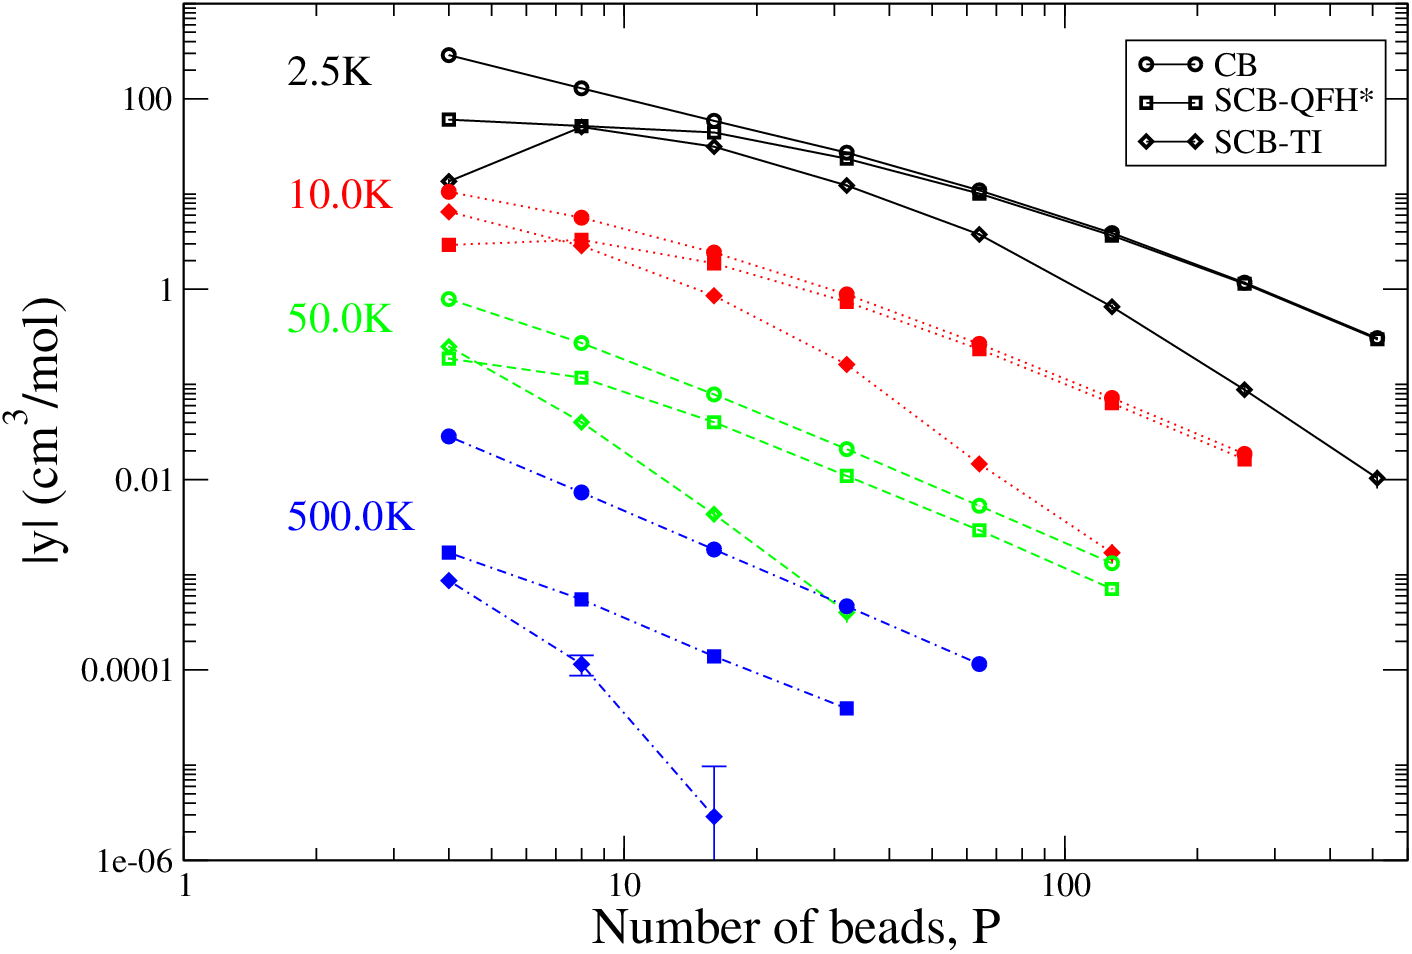
\includegraphics[scale=0.3,keepaspectratio]{Chapter-3/Figures/shMagVsP.png}
        \caption{Convergence factor, $\protect y = [\Gamma(P,u) - \Gamma(P/2,u)]$ as a function of number of beads $\protect P$. Symbols alternate filled or open with each temperature and indicate: classical-beads (CB) approach (circles); SCB-QFH* (squares); SCB-TI (diamonds). Temperatures are $\protect T = 2.5~$K (black open symbols connected by solid lines); $\protect T = 10.0~$K (red filled symbols connected by dotted lines); $\protect T = 50.0~$K (green open symbols connected by dashed lines); $\protect T = 500.0~$K (blue filled symbols connected by dash-dot lines). Confidence limits (68\%) are smaller than the symbol sizes except where shown.} \label{shMag}
    \end{figure}

    To assess the performance of SCB-QFH* and SCB-TI approaches against the CB approach in terms of achieving better precision, we plot the ratios of uncertainty of the quantity $y = [\Gamma(P,u) - \Gamma(P/2,u)]$, i.e. we plot $\sigma_y$(SCB-QFH*)/$\sigma_y$(CB) and $\sigma_y$(SCB-TI)/$\sigma_y$(CB) in Fig. \ref{uncRatios}. In order to make a fair comparison, we use the uncertainties due to the same number of MC steps ($1\times10^6$) for each case. In Fig. \ref{uncRatios} we observe that SCB-TI has a consistently lower uncertainty ratio than SCB-QFH*  for all $P$ except for $P$ = 4, where the $T$ = 2.5 and 5.0 K results for SCB-QFH* have slightly lower values. At these low temperatures, since $P > 4$ almost always, we do not worry too much about SCB-QFH* having lower uncertainty ratios because it does not affect the uncertainty of the overall result that much, and also because the values are only slightly lower. The ratio for SCB-QFH* is almost always greater than 1, suggesting that it is not expected to give better precision when compared to CB for most cases. For the cases where the SCB-QFH* ratio is less than 1, i.e. $T$ = 2.5 K and $P \le$ 128, we expect it to give better precision. The ratio for SCB-TI is almost always less than 1, suggesting that it is expected to give better precision when compared to CB for most cases. For the cases where the SCB-TI ratio is greater than 1, i.e. $T$ = 10.0 K and $P \le 8$, the magnitude is only marginally greater; as explained earlier, usually $P > 8$ is needed for accurate results when $T$ = 10.0 K.
    \begin{figure}
        \centering
        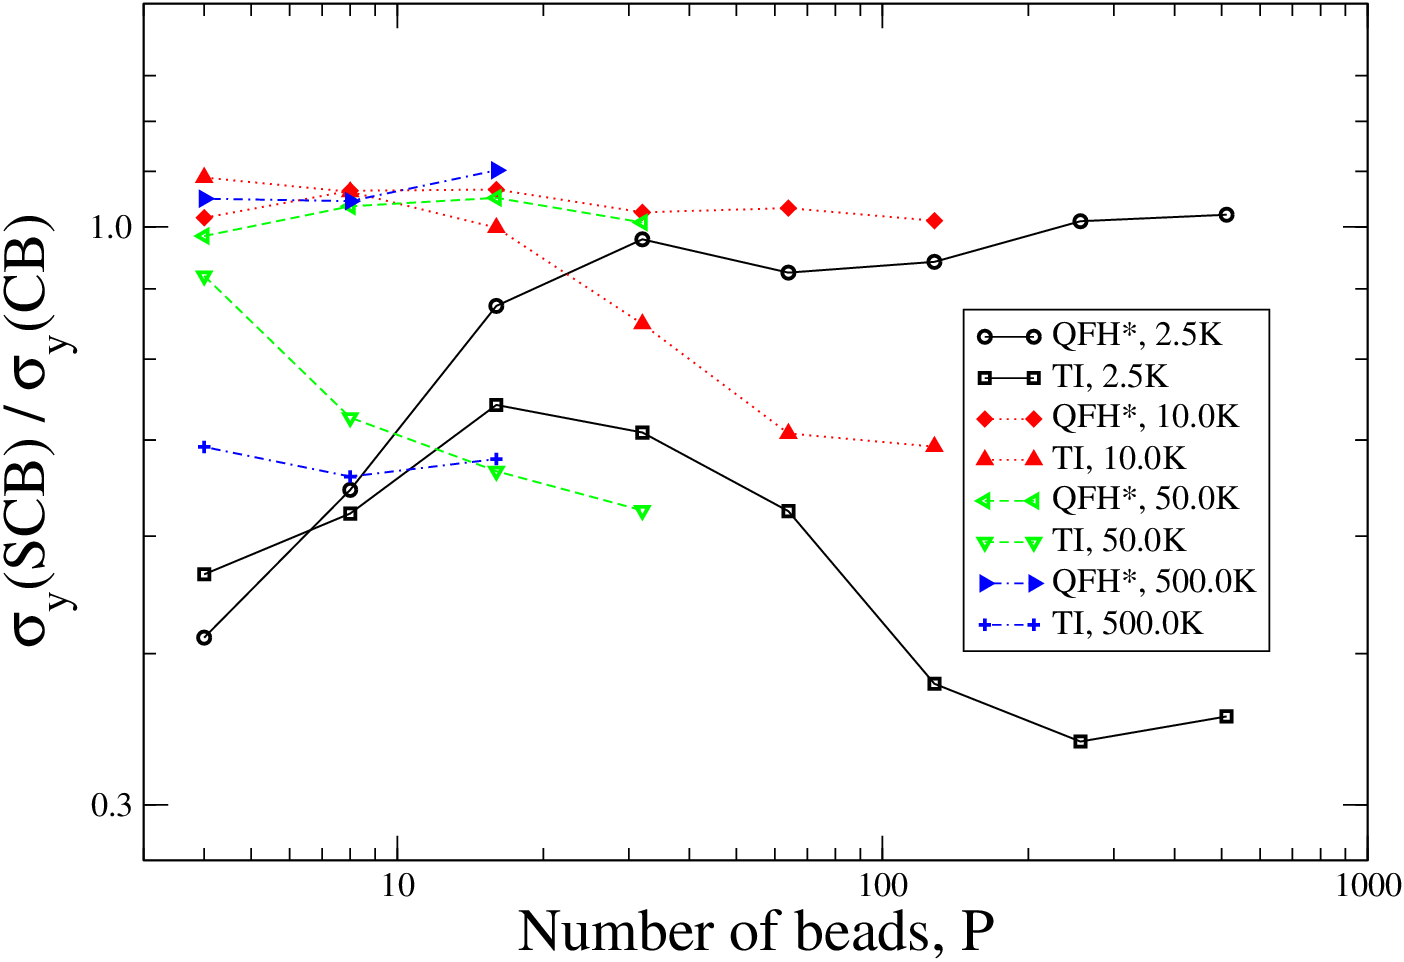
\includegraphics[scale=0.3,keepaspectratio]{Chapter-3/Figures/uncRatiosOct19.png}
        \caption{Uncertainty ratio of the convergence factor $\sigma_y (\text{SCB}) / \sigma_y (\text{CB})$, where $y = [\Gamma(P,u) - \Gamma(P/2,u)]$, as a function of number of beads $P$.}\label{uncRatios}
    \end{figure}

    To assess the performance of SCB-QFH* and SCB-TI approaches against the CB approach in terms of the uncertainty achieved for a given period of time, in Fig. \ref{uncB21Hr}we plot the ratios of best-case uncertainties of the quantum second virial coefficient values, i.e., $\sigma B_2 (\text{SCB-QFH*})/\sigma B_2 (\text{CB})$ and $\sigma B_2 (\text{SCB-QFH*} )/\sigma B_2 (\text{CB})$ that would result if we used the best possible decompositions of each of the approaches and were only allowed a total simulation time of 1h per approach. Such an estimation of the best-case uncertainty for a total simulation time of 1 h is possible as a result of performing longer simulations of each of the fragments that form the decomposition (see Shaul et al. \cite{Shaul2012} for more details). We again observe that in Fig. \ref{uncB21Hr}, the SCB-TI approach has a lower uncertainty ratio than SCB-QFH* for all temperatures considered. Also, the ratio of SCB-TI is slightly less than 1 for most cases while that of SCB-QFH* is always greater than 1. This suggests that decomposition for the SCB-QFH* approach is expected to yield larger uncertainties for the quantum virial coefficient, compared to that of CB and SCB-TI approaches. The decomposition for the SCB-TI approach seems to be performing better than the SCB-QFH* approach, especially at lower temperatures, which is desirable because we normally tend to use large $P$ at these temperatures. Even in the cases where the SCB-TI ratio is greater than 1, it is only marginally greater and therefore it may be considered acceptable.
    \begin{figure}
        \centering
        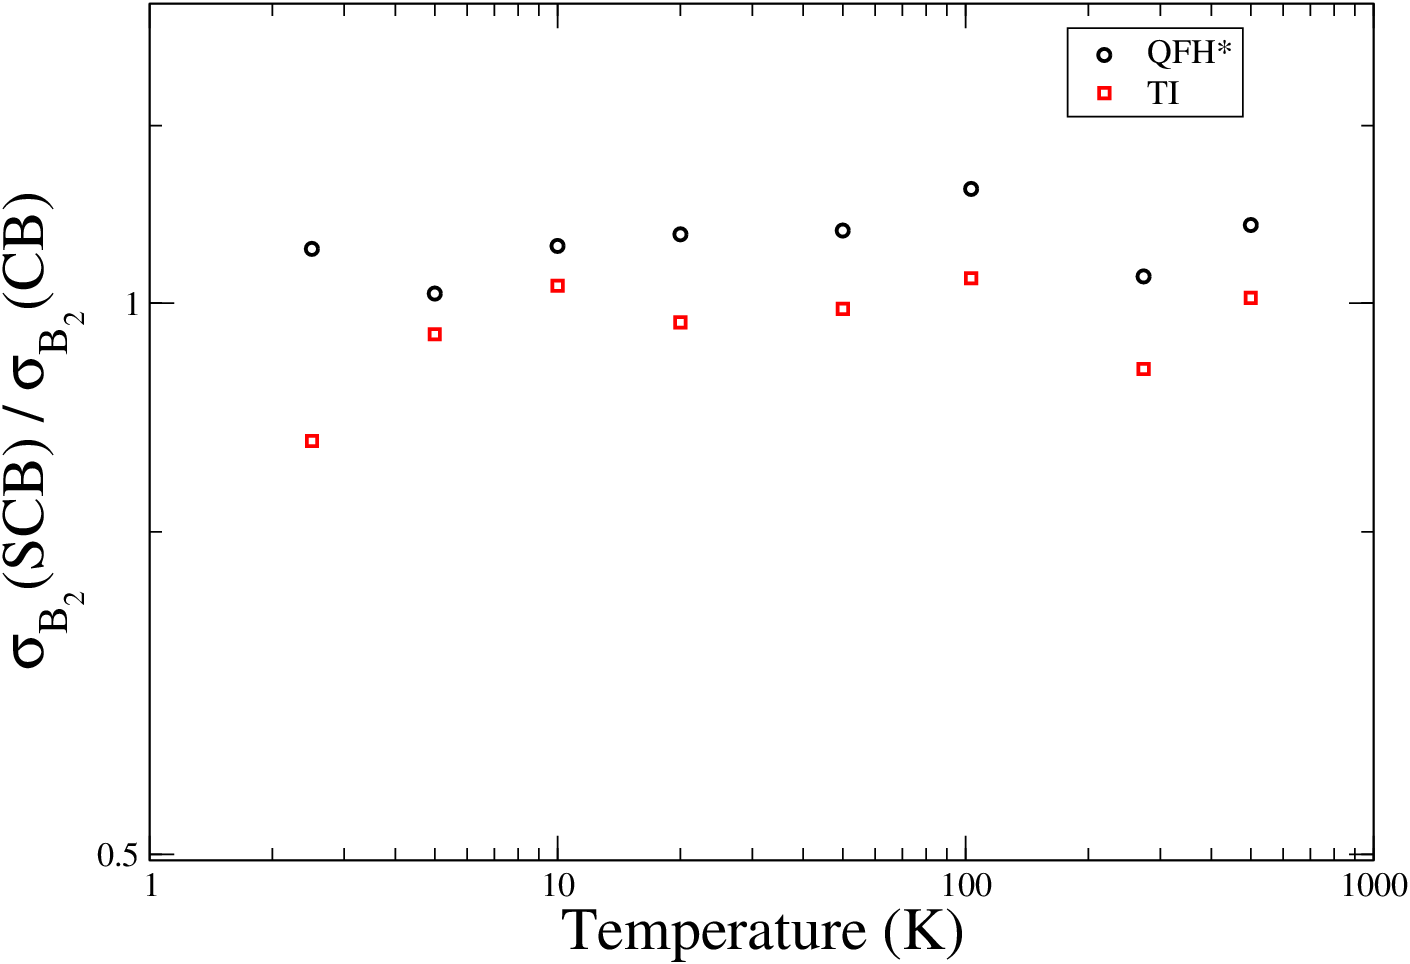
\includegraphics[scale=0.3,keepaspectratio]{Chapter-3/Figures/uncB21Hr.png}
        \caption{Uncertainty ratio $\protect \sigma_{B_2}{\rm(SCB)}/\sigma_{B_2}{\rm{(CB)}}$ as a function of temperature, for a fixed total computation time of 1 CPU-hour.} \label{uncB21Hr}
    \end{figure}

    \section{Conclusions}
    \label{sec:heConclusion}
        We have implemented the PIMC method with two approaches based on semi-classical beads (SCB-QFH*,SCB-TI) and MSMC to compute more precise quantum virial coefficients for helium-4. The SCB results agree well with CB results as they are within statistical uncertainties of each other. The decomposition algorithm of Shaul et al.~\cite{Shaul2012} was implemented to achieve better efficiency of quantum virial coefficient calculations. We observed similar trends in decompositions of simulations in our SCB based approaches as was the case for the CB approach. For lower temperatures, the approximation $u^{\rm simple}$ to $u$ for finite $P$ is chosen as the preliminary approximation. As the temperature increases, the preliminary approximation preferred is the semi-classical approximation to $u^{\rm simple}$, and for high temperatures the semi-classical approximation to $u$ is preferred. Having chosen the preliminary approximation, the decomposition algorithm spends maximum time in the first step and the amount of time spent per step gradually decreases for subsequent steps. This is because the subsequent steps involve more computationally expensive calculations (either by shifting to $u$ from its semi-classical approximation, or by doubling $P$ from the previous step, or by shifting to the full potential $u$ from $u^{\rm simple}$) and by design, these steps also yield better and better precision. The decomposition algorithm was designed to allocate computational effort proportional to the difficulty of the computation, which is defined as (error~$\times$~uncertainty). The SCB-QFH* and SCB-TI approaches have comparable and better uncertainties respectively, for the steps that involve computing $[\Gamma(P,u) - \Gamma(P/2,u)]$ or $[\Gamma(P,u^{\rm simple}) - \Gamma(P/2,u^{\rm simple})]$. Since these steps involve significant computational costs and relatively low uncertainties, the amount of effort dedicated for them is lower, attenuating the effect of any efficiency brought to their calculation. As a result, the improvement of the precision of the resulting virial coefficient is only marginal. We note that if the decomposition algorithm is not being used, either because it is non-trivial to apply, or because virial coefficients are not being computed, the SCB-TI approach performs much better than both SCB-QFH* and CB approaches, which is what we would expect anyway from the use of a higher order propagator.

        In summary, we found the following order for the rate of convergence with respect to number of beads $P$: SCB-TI $>$ SCB-QFH* $>$ CB. We expect a similar trend for the rate of convergence with respect to $P$ for higher order coefficients as well, because of the use of the higher order TI propagator. The order for precision was found to be: SCB-TI $>$ SCB-QFH*. Compared to CB, QFH* is always worse but only marginally so; TI is almost always better and only marginally worse for a few temperatures. We expected a trend similar to the rate of convergence with $P$ for the precision as well, even for $B_2$ calculations. Since this was not what we observed, partially due to the decomposition algorithm, an understanding of the order of precision for higher order coefficients for the SCB based approaches compared to CB approach would require further investigation. However, we do expect the order between SCB based approaches to remain the same, i.e., SCB-TI $>$ SCB-QFH*.
